% Options for packages loaded elsewhere
\PassOptionsToPackage{unicode}{hyperref}
\PassOptionsToPackage{hyphens}{url}
%
\documentclass[
]{article}
\usepackage{lmodern}
\usepackage{amsmath}
\usepackage{ifxetex,ifluatex}
\ifnum 0\ifxetex 1\fi\ifluatex 1\fi=0 % if pdftex
  \usepackage[T1]{fontenc}
  \usepackage[utf8]{inputenc}
  \usepackage{textcomp} % provide euro and other symbols
  \usepackage{amssymb}
\else % if luatex or xetex
  \usepackage{unicode-math}
  \defaultfontfeatures{Scale=MatchLowercase}
  \defaultfontfeatures[\rmfamily]{Ligatures=TeX,Scale=1}
\fi
% Use upquote if available, for straight quotes in verbatim environments
\IfFileExists{upquote.sty}{\usepackage{upquote}}{}
\IfFileExists{microtype.sty}{% use microtype if available
  \usepackage[]{microtype}
  \UseMicrotypeSet[protrusion]{basicmath} % disable protrusion for tt fonts
}{}
\makeatletter
\@ifundefined{KOMAClassName}{% if non-KOMA class
  \IfFileExists{parskip.sty}{%
    \usepackage{parskip}
  }{% else
    \setlength{\parindent}{0pt}
    \setlength{\parskip}{6pt plus 2pt minus 1pt}}
}{% if KOMA class
  \KOMAoptions{parskip=half}}
\makeatother
\usepackage{xcolor}
\IfFileExists{xurl.sty}{\usepackage{xurl}}{} % add URL line breaks if available
\IfFileExists{bookmark.sty}{\usepackage{bookmark}}{\usepackage{hyperref}}
\hypersetup{
  pdftitle={Gestion de Portefeuille},
  pdfauthor={Paul Giraud , Kouamé YAO \& Loïc Turounet},
  hidelinks,
  pdfcreator={LaTeX via pandoc}}
\urlstyle{same} % disable monospaced font for URLs
\usepackage[margin=1in]{geometry}
\usepackage{color}
\usepackage{fancyvrb}
\newcommand{\VerbBar}{|}
\newcommand{\VERB}{\Verb[commandchars=\\\{\}]}
\DefineVerbatimEnvironment{Highlighting}{Verbatim}{commandchars=\\\{\}}
% Add ',fontsize=\small' for more characters per line
\usepackage{framed}
\definecolor{shadecolor}{RGB}{248,248,248}
\newenvironment{Shaded}{\begin{snugshade}}{\end{snugshade}}
\newcommand{\AlertTok}[1]{\textcolor[rgb]{0.94,0.16,0.16}{#1}}
\newcommand{\AnnotationTok}[1]{\textcolor[rgb]{0.56,0.35,0.01}{\textbf{\textit{#1}}}}
\newcommand{\AttributeTok}[1]{\textcolor[rgb]{0.77,0.63,0.00}{#1}}
\newcommand{\BaseNTok}[1]{\textcolor[rgb]{0.00,0.00,0.81}{#1}}
\newcommand{\BuiltInTok}[1]{#1}
\newcommand{\CharTok}[1]{\textcolor[rgb]{0.31,0.60,0.02}{#1}}
\newcommand{\CommentTok}[1]{\textcolor[rgb]{0.56,0.35,0.01}{\textit{#1}}}
\newcommand{\CommentVarTok}[1]{\textcolor[rgb]{0.56,0.35,0.01}{\textbf{\textit{#1}}}}
\newcommand{\ConstantTok}[1]{\textcolor[rgb]{0.00,0.00,0.00}{#1}}
\newcommand{\ControlFlowTok}[1]{\textcolor[rgb]{0.13,0.29,0.53}{\textbf{#1}}}
\newcommand{\DataTypeTok}[1]{\textcolor[rgb]{0.13,0.29,0.53}{#1}}
\newcommand{\DecValTok}[1]{\textcolor[rgb]{0.00,0.00,0.81}{#1}}
\newcommand{\DocumentationTok}[1]{\textcolor[rgb]{0.56,0.35,0.01}{\textbf{\textit{#1}}}}
\newcommand{\ErrorTok}[1]{\textcolor[rgb]{0.64,0.00,0.00}{\textbf{#1}}}
\newcommand{\ExtensionTok}[1]{#1}
\newcommand{\FloatTok}[1]{\textcolor[rgb]{0.00,0.00,0.81}{#1}}
\newcommand{\FunctionTok}[1]{\textcolor[rgb]{0.00,0.00,0.00}{#1}}
\newcommand{\ImportTok}[1]{#1}
\newcommand{\InformationTok}[1]{\textcolor[rgb]{0.56,0.35,0.01}{\textbf{\textit{#1}}}}
\newcommand{\KeywordTok}[1]{\textcolor[rgb]{0.13,0.29,0.53}{\textbf{#1}}}
\newcommand{\NormalTok}[1]{#1}
\newcommand{\OperatorTok}[1]{\textcolor[rgb]{0.81,0.36,0.00}{\textbf{#1}}}
\newcommand{\OtherTok}[1]{\textcolor[rgb]{0.56,0.35,0.01}{#1}}
\newcommand{\PreprocessorTok}[1]{\textcolor[rgb]{0.56,0.35,0.01}{\textit{#1}}}
\newcommand{\RegionMarkerTok}[1]{#1}
\newcommand{\SpecialCharTok}[1]{\textcolor[rgb]{0.00,0.00,0.00}{#1}}
\newcommand{\SpecialStringTok}[1]{\textcolor[rgb]{0.31,0.60,0.02}{#1}}
\newcommand{\StringTok}[1]{\textcolor[rgb]{0.31,0.60,0.02}{#1}}
\newcommand{\VariableTok}[1]{\textcolor[rgb]{0.00,0.00,0.00}{#1}}
\newcommand{\VerbatimStringTok}[1]{\textcolor[rgb]{0.31,0.60,0.02}{#1}}
\newcommand{\WarningTok}[1]{\textcolor[rgb]{0.56,0.35,0.01}{\textbf{\textit{#1}}}}
\usepackage{longtable,booktabs}
\usepackage{calc} % for calculating minipage widths
% Correct order of tables after \paragraph or \subparagraph
\usepackage{etoolbox}
\makeatletter
\patchcmd\longtable{\par}{\if@noskipsec\mbox{}\fi\par}{}{}
\makeatother
% Allow footnotes in longtable head/foot
\IfFileExists{footnotehyper.sty}{\usepackage{footnotehyper}}{\usepackage{footnote}}
\makesavenoteenv{longtable}
\usepackage{graphicx}
\makeatletter
\def\maxwidth{\ifdim\Gin@nat@width>\linewidth\linewidth\else\Gin@nat@width\fi}
\def\maxheight{\ifdim\Gin@nat@height>\textheight\textheight\else\Gin@nat@height\fi}
\makeatother
% Scale images if necessary, so that they will not overflow the page
% margins by default, and it is still possible to overwrite the defaults
% using explicit options in \includegraphics[width, height, ...]{}
\setkeys{Gin}{width=\maxwidth,height=\maxheight,keepaspectratio}
% Set default figure placement to htbp
\makeatletter
\def\fps@figure{htbp}
\makeatother
\setlength{\emergencystretch}{3em} % prevent overfull lines
\providecommand{\tightlist}{%
  \setlength{\itemsep}{0pt}\setlength{\parskip}{0pt}}
\setcounter{secnumdepth}{-\maxdimen} % remove section numbering
\usepackage[utf8]{inputenc}
\usepackage{amsmath}
\usepackage{amsfonts}
\usepackage{amssymb}
\ifluatex
  \usepackage{selnolig}  % disable illegal ligatures
\fi

\title{Gestion de Portefeuille}
\usepackage{etoolbox}
\makeatletter
\providecommand{\subtitle}[1]{% add subtitle to \maketitle
  \apptocmd{\@title}{\par {\large #1 \par}}{}{}
}
\makeatother
\subtitle{TP-1: Analyse du CAC40}
\author{Paul Giraud , Kouamé YAO \& Loïc Turounet}
\date{Version: 27 fév 2022}

\begin{document}
\maketitle

\begin{Shaded}
\begin{Highlighting}[]
\FunctionTok{library}\NormalTok{(lubridate)}
\FunctionTok{library}\NormalTok{(Hmisc)}
\FunctionTok{library}\NormalTok{(tseries)}
\FunctionTok{library}\NormalTok{(timeSeries)}
\FunctionTok{library}\NormalTok{(corrplot)}
\FunctionTok{library}\NormalTok{(zoo)}

\NormalTok{get.src.folder }\OtherTok{\textless{}{-}} \ControlFlowTok{function}\NormalTok{() \{}
  \FunctionTok{path.expand}\NormalTok{(}\StringTok{"../GP/src"}\NormalTok{)}
\NormalTok{\}}

\NormalTok{get.data.folder }\OtherTok{\textless{}{-}} \ControlFlowTok{function}\NormalTok{() \{}
  \FunctionTok{path.expand}\NormalTok{(}\StringTok{"../GP/data"}\NormalTok{)}
\NormalTok{\}}

\FunctionTok{source}\NormalTok{(}\FunctionTok{file.path}\NormalTok{(}\FunctionTok{get.src.folder}\NormalTok{(), }\StringTok{\textquotesingle{}utils.R\textquotesingle{}}\NormalTok{))}
\FunctionTok{source}\NormalTok{(}\FunctionTok{file.path}\NormalTok{(}\FunctionTok{get.src.folder}\NormalTok{(), }\StringTok{\textquotesingle{}FileUtils.R\textquotesingle{}}\NormalTok{))}
\end{Highlighting}
\end{Shaded}

\hypertarget{les-donnuxe9es}{%
\subsection{Les données}\label{les-donnuxe9es}}

On charge les séries de rendements pour l'indice et les composants de
l'indice.

\begin{Shaded}
\begin{Highlighting}[]
\NormalTok{ts.all }\OtherTok{\textless{}{-}} \FunctionTok{get.all.ts}\NormalTok{(}\StringTok{\textquotesingle{}CAC40\textquotesingle{}}\NormalTok{, }\AttributeTok{tickers=}\ConstantTok{NULL}\NormalTok{, }\AttributeTok{returns =} \ConstantTok{TRUE}\NormalTok{,}
  \AttributeTok{dt.start =} \FunctionTok{dmy}\NormalTok{(}\StringTok{\textquotesingle{}01Jul2007\textquotesingle{}}\NormalTok{), }\AttributeTok{combine =}\NormalTok{ T)}

\CommentTok{\# bad data for Valeo}
\NormalTok{ts.all }\OtherTok{\textless{}{-}}\NormalTok{ ts.all[,}\SpecialCharTok{{-}}\DecValTok{17}\NormalTok{]}

\CommentTok{\# keep good data window}
\NormalTok{ts.all }\OtherTok{\textless{}{-}} \FunctionTok{window}\NormalTok{(ts.all, }\FunctionTok{dmy}\NormalTok{(}\StringTok{\textquotesingle{}01Jul2007\textquotesingle{}}\NormalTok{), }
                 \FunctionTok{dmy}\NormalTok{(}\StringTok{\textquotesingle{}01Jan2009\textquotesingle{}}\NormalTok{))}

\CommentTok{\# merge with cac40 index}
\NormalTok{cac.index }\OtherTok{\textless{}{-}} \FunctionTok{get.ts}\NormalTok{(}\StringTok{\textquotesingle{}fchi\textquotesingle{}}\NormalTok{, }\StringTok{\textquotesingle{}CAC40\textquotesingle{}}\NormalTok{)}

\NormalTok{cac.ret }\OtherTok{\textless{}{-}} \FunctionTok{returns}\NormalTok{(cac.index)}
\FunctionTok{names}\NormalTok{(cac.ret) }\OtherTok{\textless{}{-}} \StringTok{\textquotesingle{}CAC40\textquotesingle{}}
\NormalTok{ts.all }\OtherTok{\textless{}{-}} \FunctionTok{removeNA}\NormalTok{(}\FunctionTok{cbind}\NormalTok{(ts.all, cac.ret))}
\end{Highlighting}
\end{Shaded}

\begin{Shaded}
\begin{Highlighting}[]
\FunctionTok{plot}\NormalTok{(ts.all[, }\FunctionTok{c}\NormalTok{(}\DecValTok{1}\NormalTok{,}\DecValTok{2}\NormalTok{,}\DecValTok{3}\NormalTok{)], }\AttributeTok{main=}\StringTok{\textquotesingle{}Rendement quotidien\textquotesingle{}}\NormalTok{)}
\end{Highlighting}
\end{Shaded}

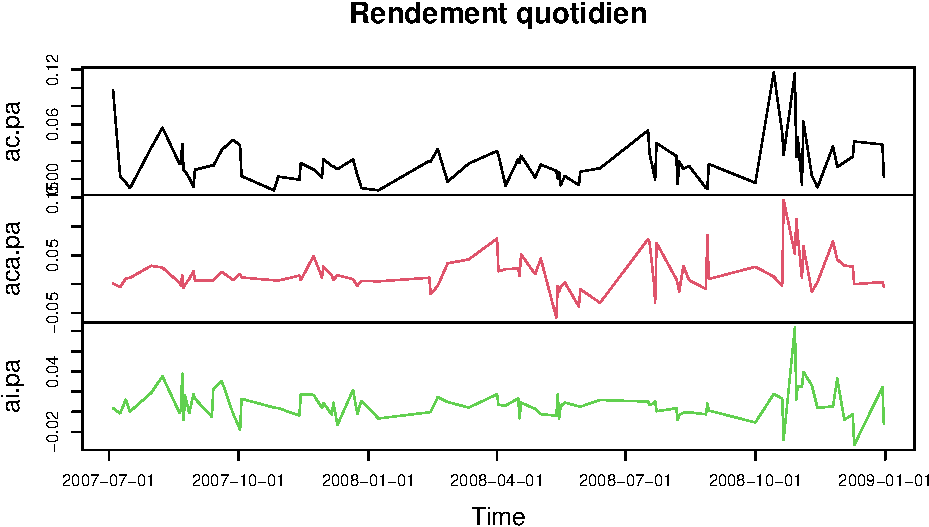
\includegraphics{TP-1_files/figure-latex/plot-cac-1-1.pdf}

Puis on filtre les points suspects: rendements supérieur à 8 s.d.

\begin{Shaded}
\begin{Highlighting}[]
  \CommentTok{\# flag bad data points: \textgreater{} * \textbackslash{}sigma}
\NormalTok{  good.limit }\OtherTok{\textless{}{-}} \DecValTok{8}\SpecialCharTok{*}\FunctionTok{apply}\NormalTok{(ts.all, }\DecValTok{2}\NormalTok{, sd)}
  
\NormalTok{  ts.bad }\OtherTok{\textless{}{-}}\NormalTok{ ts.all}\SpecialCharTok{*}\ConstantTok{FALSE}
  \ControlFlowTok{for}\NormalTok{(j }\ControlFlowTok{in} \FunctionTok{seq}\NormalTok{(}\FunctionTok{ncol}\NormalTok{(ts.bad))) \{}
\NormalTok{    ts.bad[,j] }\OtherTok{\textless{}{-}} \FunctionTok{abs}\NormalTok{(ts.all[,j]) }\SpecialCharTok{\textgreater{}}\NormalTok{ good.limit[j]}
\NormalTok{  \}}
\NormalTok{  good.index }\OtherTok{\textless{}{-}} \SpecialCharTok{!}\FunctionTok{apply}\NormalTok{(ts.bad,}\DecValTok{1}\NormalTok{,any)}
\NormalTok{  ts.all }\OtherTok{\textless{}{-}}\NormalTok{ ts.all[good.index,]}
\end{Highlighting}
\end{Shaded}

Finalement, on calcule les rendements hebdomadaires:

\begin{Shaded}
\begin{Highlighting}[]
  \CommentTok{\# aggregate returns by week}
\NormalTok{  by }\OtherTok{\textless{}{-}} \FunctionTok{timeSequence}\NormalTok{(}\AttributeTok{from=}\FunctionTok{start}\NormalTok{(ts.all), }
                     \AttributeTok{to=}\FunctionTok{end}\NormalTok{(ts.all), }\AttributeTok{by=}\StringTok{\textquotesingle{}week\textquotesingle{}}\NormalTok{)}
\NormalTok{  ts.all.weekly }\OtherTok{\textless{}{-}} \FunctionTok{aggregate}\NormalTok{(ts.all, by, sum)}

\NormalTok{  ts.stocks }\OtherTok{\textless{}{-}}\NormalTok{ ts.all.weekly[,}\SpecialCharTok{{-}}\DecValTok{40}\NormalTok{]}
\NormalTok{  ts.index }\OtherTok{\textless{}{-}}\NormalTok{ ts.all.weekly[,}\DecValTok{40}\NormalTok{]}
\end{Highlighting}
\end{Shaded}

\begin{Shaded}
\begin{Highlighting}[]
\FunctionTok{plot}\NormalTok{(ts.index, }\AttributeTok{main=}\StringTok{\textquotesingle{}Rendement hebdomadaire de l}\SpecialCharTok{\textbackslash{}\textquotesingle{}}\StringTok{indice CAC40\textquotesingle{}}\NormalTok{)}
\end{Highlighting}
\end{Shaded}

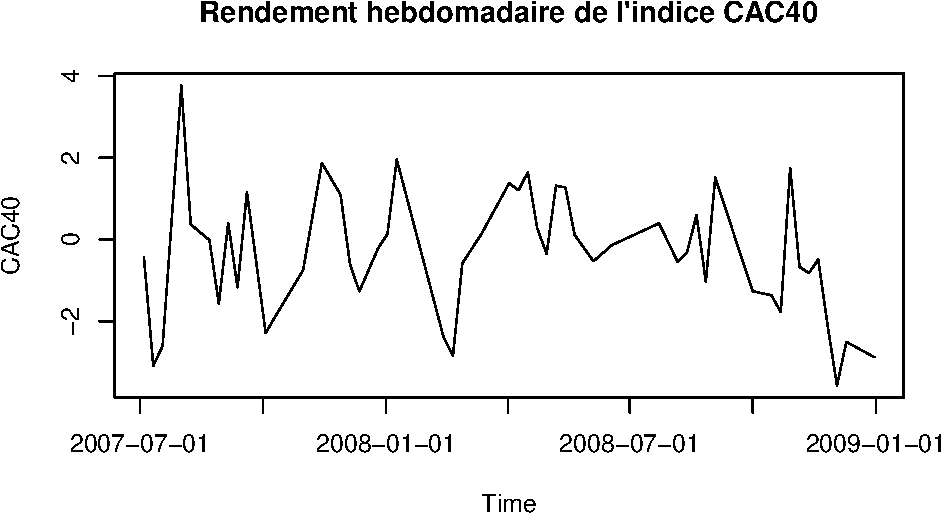
\includegraphics{TP-1_files/figure-latex/plot-cac-2-1.pdf}

\hypertarget{calcul-de-correlation}{%
\subsection{Calcul de correlation}\label{calcul-de-correlation}}

\begin{itemize}
\tightlist
\item
  Calculer la matrice de corrélation des actions de l'indice.
\end{itemize}

\begin{Shaded}
\begin{Highlighting}[]
\NormalTok{assets.cor }\OtherTok{=} \FunctionTok{cor}\NormalTok{(ts.stocks)}
\FunctionTok{corrplot}\NormalTok{(assets.cor, }\AttributeTok{type=}\StringTok{"upper"}\NormalTok{, }\AttributeTok{cl.pos =} \StringTok{"r"}\NormalTok{, }\AttributeTok{tl.pos =} \StringTok{"lt"}\NormalTok{, }
         \AttributeTok{tl.cex =} \FloatTok{0.5}\NormalTok{, }\AttributeTok{title=} \StringTok{"Matrice de Corrélation des composants de l}\SpecialCharTok{\textbackslash{}\textquotesingle{}}\StringTok{indice CAC 40"}\NormalTok{, }\AttributeTok{mar=}\FunctionTok{c}\NormalTok{(}\DecValTok{0}\NormalTok{,}\DecValTok{0}\NormalTok{,}\DecValTok{1}\NormalTok{,}\DecValTok{0}\NormalTok{))}
\end{Highlighting}
\end{Shaded}

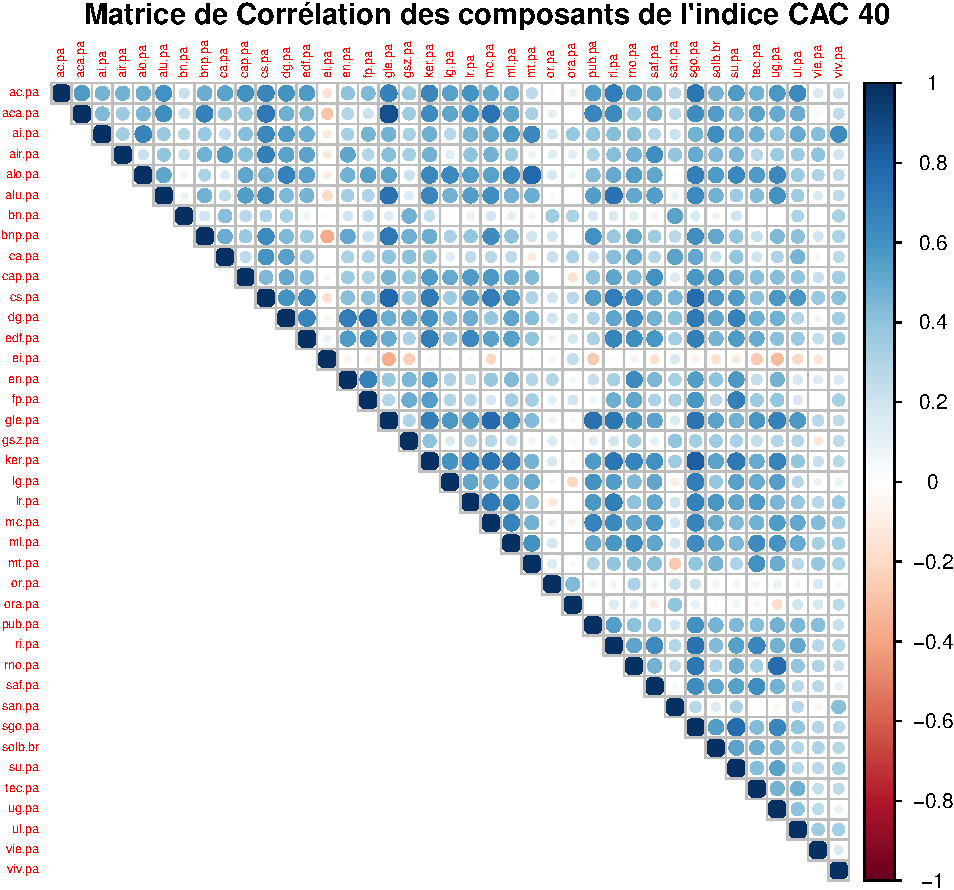
\includegraphics{TP-1_files/figure-latex/correl-matrix-1.pdf}

\begin{itemize}
\tightlist
\item
  Rechercher des actions fortement corrélées et d'autres qui semblent
  indépendantes. Justifier ces observations en considérant la nature des
  entreprises.
\end{itemize}

\hypertarget{recherche-des-titres-fortement-corruxe9luxe9s}{%
\subsubsection{Recherche des titres fortement
corrélés}\label{recherche-des-titres-fortement-corruxe9luxe9s}}

\begin{itemize}
\tightlist
\item
  On considera que les actions sont fortement corrélées lorsque la
  corrélation entre les deux actifs est supérieure à 0,7.
\end{itemize}

\begin{Shaded}
\begin{Highlighting}[]
\NormalTok{min }\OtherTok{\textless{}{-}} \FloatTok{0.7}
\NormalTok{highCorr }\OtherTok{\textless{}{-}} \FunctionTok{data.frame}\NormalTok{(}\AttributeTok{Ticker1=}\FunctionTok{character}\NormalTok{(}\DecValTok{0}\NormalTok{), }
                       \AttributeTok{Ticker2=}\FunctionTok{character}\NormalTok{(}\DecValTok{0}\NormalTok{), }
                       \AttributeTok{Correlation=}\FunctionTok{numeric}\NormalTok{(}\DecValTok{0}\NormalTok{), }
                       \AttributeTok{stringsAsFactors=}\ConstantTok{FALSE}\NormalTok{)}
\NormalTok{temp.assets.cor }\OtherTok{\textless{}{-}}\NormalTok{ assets.cor}
\FunctionTok{diag}\NormalTok{(temp.assets.cor) }\OtherTok{\textless{}{-}} \DecValTok{0}
\ControlFlowTok{while}\NormalTok{ (}\FunctionTok{sum}\NormalTok{(temp.assets.cor}\SpecialCharTok{\textgreater{}}\NormalTok{min)}\SpecialCharTok{\textgreater{}}\DecValTok{1}\NormalTok{) \{}
\NormalTok{  maxval }\OtherTok{\textless{}{-}} \FunctionTok{max}\NormalTok{(temp.assets.cor)}
\NormalTok{  max }\OtherTok{\textless{}{-}} \FunctionTok{which}\NormalTok{(temp.assets.cor}\SpecialCharTok{==}\NormalTok{maxval, }\AttributeTok{arr.ind=}\ConstantTok{TRUE}\NormalTok{)[}\DecValTok{1}\NormalTok{,]}
\NormalTok{  highCorr }\OtherTok{\textless{}{-}} \FunctionTok{rbind}\NormalTok{(highCorr, }\FunctionTok{data.frame}\NormalTok{(}
    \AttributeTok{Ticker1=}\FunctionTok{rownames}\NormalTok{(temp.assets.cor)[max[}\DecValTok{1}\NormalTok{]], }
    \AttributeTok{Ticker2=}\FunctionTok{colnames}\NormalTok{(temp.assets.cor)[max[}\DecValTok{2}\NormalTok{]], }
    \AttributeTok{Correlation=}\NormalTok{maxval))}
\NormalTok{  temp.assets.cor[max[}\DecValTok{1}\NormalTok{],] }\OtherTok{\textless{}{-}} \DecValTok{0}
\NormalTok{  temp.assets.cor[,max[}\DecValTok{1}\NormalTok{]] }\OtherTok{\textless{}{-}} \DecValTok{0}
\NormalTok{  temp.assets.cor[max[}\DecValTok{2}\NormalTok{],] }\OtherTok{\textless{}{-}} \DecValTok{0}
\NormalTok{  temp.assets.cor[,max[}\DecValTok{2}\NormalTok{]] }\OtherTok{\textless{}{-}} \DecValTok{0}
\NormalTok{\}}

\NormalTok{caption }\OtherTok{\textless{}{-}} \FunctionTok{paste}\NormalTok{(}\StringTok{"CAC40 corrélation forte (supérieure à "}\NormalTok{, }
                 \FunctionTok{toString}\NormalTok{(min),}\StringTok{")"}\NormalTok{)}
\NormalTok{knitr}\SpecialCharTok{::}\FunctionTok{kable}\NormalTok{(highCorr, }
             \AttributeTok{col.names=}\FunctionTok{c}\NormalTok{(}\StringTok{"Ticker1"}\NormalTok{, }\StringTok{"Ticker2"}\NormalTok{, }\StringTok{"Corrélation"}\NormalTok{), }
             \AttributeTok{caption=}\NormalTok{caption,}
             \AttributeTok{digits=}\DecValTok{2}\NormalTok{, }\AttributeTok{booktab=}\ConstantTok{TRUE}\NormalTok{, }\AttributeTok{row.names=}\ConstantTok{FALSE}\NormalTok{)}
\end{Highlighting}
\end{Shaded}

\begin{longtable}[]{@{}llr@{}}
\caption{CAC40 corrélation forte (supérieure à 0.7 )}\tabularnewline
\toprule
Ticker1 & Ticker2 & Corrélation\tabularnewline
\midrule
\endfirsthead
\toprule
Ticker1 & Ticker2 & Corrélation\tabularnewline
\midrule
\endhead
gle.pa & aca.pa & 0.88\tabularnewline
sgo.pa & ker.pa & 0.83\tabularnewline
mt.pa & alo.pa & 0.78\tabularnewline
ug.pa & rno.pa & 0.77\tabularnewline
fp.pa & dg.pa & 0.75\tabularnewline
ri.pa & alu.pa & 0.74\tabularnewline
mc.pa & lr.pa & 0.71\tabularnewline
\bottomrule
\end{longtable}

\hypertarget{table-1---forte-corruxe9lation}{%
\subsubsection{Table 1 - Forte
corrélation}\label{table-1---forte-corruxe9lation}}

On remarque que les fortes corrélations sont justifiées par
l'appartenance à un même secteur économique:

\begin{itemize}
\tightlist
\item
  GLE (Société Générale), ACA (Credit Agricole) sont deux compagnies du
  même secteur (banques françaises)
\item
  SGO (Cie de Saint-Gobain), KER (Kering) matérieux de construction et
  luxe
\item
  MT (ArcelorMittal), ALO (Alstom) sidérurgie et transports ferroviaires
\item
  UG (Peugeot), RNO (Renault) sont deux compagnies du même secteur
  (automobile français)
\item
  FP (Total), DG (Vinci) énergie et concessions/construction
\item
  RI (Pernod Ricard), ALU (Alcatel-Lucent) distribution de vin et
  spiritueux et télécommunications
\item
  MC (LVMH), LR (Legrand) luxe et infracstructures électrique
\end{itemize}

\hypertarget{recherche-des-titres-nuxe9gativement-corruxe9luxe9s}{%
\subsubsection{Recherche des titres négativement
corrélés}\label{recherche-des-titres-nuxe9gativement-corruxe9luxe9s}}

\begin{Shaded}
\begin{Highlighting}[]
\NormalTok{max }\OtherTok{\textless{}{-}} \SpecialCharTok{{-}}\FloatTok{0.05}
\NormalTok{lowCorr }\OtherTok{\textless{}{-}} \FunctionTok{data.frame}\NormalTok{(}\AttributeTok{v1=}\FunctionTok{character}\NormalTok{(}\DecValTok{0}\NormalTok{), }\AttributeTok{v2=}\FunctionTok{character}\NormalTok{(}\DecValTok{0}\NormalTok{), }\AttributeTok{cor=}\FunctionTok{numeric}\NormalTok{(}\DecValTok{0}\NormalTok{), }
                      \AttributeTok{stringsAsFactors=}\ConstantTok{FALSE}\NormalTok{)}
\NormalTok{temp.assets.cor }\OtherTok{\textless{}{-}}\NormalTok{ assets.cor}
\FunctionTok{diag}\NormalTok{(temp.assets.cor) }\OtherTok{\textless{}{-}} \DecValTok{0}
\ControlFlowTok{while}\NormalTok{ (}\FunctionTok{sum}\NormalTok{(temp.assets.cor}\SpecialCharTok{\textless{}}\NormalTok{max)}\SpecialCharTok{\textgreater{}}\DecValTok{1}\NormalTok{) \{}
\NormalTok{  minval }\OtherTok{\textless{}{-}} \FunctionTok{min}\NormalTok{(temp.assets.cor)}
\NormalTok{  min }\OtherTok{\textless{}{-}} \FunctionTok{which}\NormalTok{(temp.assets.cor}\SpecialCharTok{==}\NormalTok{minval, }\AttributeTok{arr.ind=}\ConstantTok{TRUE}\NormalTok{)[}\DecValTok{1}\NormalTok{,]}
\NormalTok{  lowCorr }\OtherTok{\textless{}{-}} \FunctionTok{rbind}\NormalTok{(lowCorr, }\FunctionTok{data.frame}\NormalTok{(}\AttributeTok{v1=}\FunctionTok{rownames}\NormalTok{(temp.assets.cor)[min[}\DecValTok{1}\NormalTok{]], }
                                       \AttributeTok{v2=}\FunctionTok{colnames}\NormalTok{(temp.assets.cor)[min[}\DecValTok{2}\NormalTok{]], }
                                       \AttributeTok{cor=}\NormalTok{minval))}
\NormalTok{  temp.assets.cor[min[}\DecValTok{1}\NormalTok{],] }\OtherTok{\textless{}{-}} \DecValTok{0}
\NormalTok{  temp.assets.cor[,min[}\DecValTok{1}\NormalTok{]] }\OtherTok{\textless{}{-}} \DecValTok{0}
\NormalTok{  temp.assets.cor[min[}\DecValTok{2}\NormalTok{],] }\OtherTok{\textless{}{-}} \DecValTok{0}
\NormalTok{  temp.assets.cor[,min[}\DecValTok{2}\NormalTok{]] }\OtherTok{\textless{}{-}} \DecValTok{0}
\NormalTok{\}}

\NormalTok{caption }\OtherTok{\textless{}{-}} \FunctionTok{paste}\NormalTok{(}\StringTok{"CAC40 Faible corrélation (inférieure à  "}\NormalTok{, }\FunctionTok{toString}\NormalTok{(max),}\StringTok{")"}\NormalTok{)}
\NormalTok{knitr}\SpecialCharTok{::}\FunctionTok{kable}\NormalTok{(lowCorr,}
             \AttributeTok{col.names=}\FunctionTok{c}\NormalTok{(}\StringTok{"Ticker1"}\NormalTok{, }\StringTok{"Ticker2"}\NormalTok{, }\StringTok{"Corrélation"}\NormalTok{), }
             \AttributeTok{caption=}\NormalTok{caption,}
             \AttributeTok{digits=}\DecValTok{2}\NormalTok{, }\AttributeTok{booktab=}\ConstantTok{TRUE}\NormalTok{, }\AttributeTok{row.names=}\ConstantTok{FALSE}\NormalTok{)}
\end{Highlighting}
\end{Shaded}

\begin{longtable}[]{@{}llr@{}}
\caption{CAC40 Faible corrélation (inférieure à -0.05 )}\tabularnewline
\toprule
Ticker1 & Ticker2 & Corrélation\tabularnewline
\midrule
\endfirsthead
\toprule
Ticker1 & Ticker2 & Corrélation\tabularnewline
\midrule
\endhead
ei.pa & bnp.pa & -0.37\tabularnewline
san.pa & mt.pa & -0.27\tabularnewline
ora.pa & lg.pa & -0.20\tabularnewline
vie.pa & gsz.pa & -0.13\tabularnewline
or.pa & lr.pa & -0.13\tabularnewline
saf.pa & bn.pa & -0.06\tabularnewline
\bottomrule
\end{longtable}

\hypertarget{table-2---corruxe9lation-nuxe9gative}{%
\subsubsection{Table 2 - Corrélation
négative}\label{table-2---corruxe9lation-nuxe9gative}}

Par opposition, les corrélations faibles se justifient lorsque les
entreprises ne sont pas en général du même domaine d'activité.

\begin{itemize}
\tightlist
\item
  EI (EssilorLuxottica), BNP (BNP Paribas)
\item
  SAN (Sanofi), MT (ArcelorMittal)
\item
  ORA (Orange), LG (Lafargue)
\item
  VIE (Veolia), GSZ (ENGIE)
\item
  OR (l'Oréal), Lr (Legrand)
\item
  SAF (Safran), BN (Danone)
\end{itemize}

\begin{Shaded}
\begin{Highlighting}[]
\NormalTok{epsilon }\OtherTok{\textless{}{-}} \FloatTok{0.05}
\NormalTok{lowCorr }\OtherTok{\textless{}{-}} \FunctionTok{data.frame}\NormalTok{(}\AttributeTok{v1=}\FunctionTok{character}\NormalTok{(}\DecValTok{0}\NormalTok{), }\AttributeTok{v2=}\FunctionTok{character}\NormalTok{(}\DecValTok{0}\NormalTok{), }\AttributeTok{cor=}\FunctionTok{numeric}\NormalTok{(}\DecValTok{0}\NormalTok{), }
                      \AttributeTok{stringsAsFactors=}\ConstantTok{FALSE}\NormalTok{)}
\NormalTok{temp.assets.cor }\OtherTok{\textless{}{-}}\NormalTok{ assets.cor}
\FunctionTok{diag}\NormalTok{(temp.assets.cor) }\OtherTok{\textless{}{-}} \DecValTok{100}
\ControlFlowTok{while}\NormalTok{ (}\FunctionTok{sum}\NormalTok{(}\FunctionTok{abs}\NormalTok{(temp.assets.cor)}\SpecialCharTok{\textless{}}\NormalTok{epsilon)}\SpecialCharTok{\textgreater{}}\DecValTok{1}\NormalTok{) \{}
\NormalTok{  minval }\OtherTok{\textless{}{-}} \FunctionTok{min}\NormalTok{(}\FunctionTok{abs}\NormalTok{(temp.assets.cor))}
\NormalTok{  min }\OtherTok{\textless{}{-}} \FunctionTok{which}\NormalTok{(}\FunctionTok{abs}\NormalTok{(temp.assets.cor)}\SpecialCharTok{==}\NormalTok{minval, }\AttributeTok{arr.ind=}\ConstantTok{TRUE}\NormalTok{)[}\DecValTok{1}\NormalTok{,]}
\NormalTok{  val }\OtherTok{\textless{}{-}}\NormalTok{ temp.assets.cor[min[}\DecValTok{1}\NormalTok{],min[}\DecValTok{2}\NormalTok{]]}
\NormalTok{  lowCorr }\OtherTok{\textless{}{-}} \FunctionTok{rbind}\NormalTok{(lowCorr, }\FunctionTok{data.frame}\NormalTok{(}\AttributeTok{v1=}\FunctionTok{rownames}\NormalTok{(temp.assets.cor)[min[}\DecValTok{1}\NormalTok{]], }
                                       \AttributeTok{v2=}\FunctionTok{colnames}\NormalTok{(temp.assets.cor)[min[}\DecValTok{2}\NormalTok{]], }
                                       \AttributeTok{cor=}\NormalTok{val))}
\NormalTok{  temp.assets.cor[min[}\DecValTok{1}\NormalTok{],] }\OtherTok{\textless{}{-}} \DecValTok{100}
\NormalTok{  temp.assets.cor[,min[}\DecValTok{1}\NormalTok{]] }\OtherTok{\textless{}{-}} \DecValTok{100}
\NormalTok{  temp.assets.cor[min[}\DecValTok{2}\NormalTok{],] }\OtherTok{\textless{}{-}} \DecValTok{100}
\NormalTok{  temp.assets.cor[,min[}\DecValTok{2}\NormalTok{]] }\OtherTok{\textless{}{-}} \DecValTok{100}

\NormalTok{\}}

\NormalTok{caption }\OtherTok{\textless{}{-}} \FunctionTok{paste}\NormalTok{(}\StringTok{"CAC40 corrélation (independance)"}\NormalTok{)}
\NormalTok{knitr}\SpecialCharTok{::}\FunctionTok{kable}\NormalTok{(lowCorr,}
             \AttributeTok{col.names=}\FunctionTok{c}\NormalTok{(}\StringTok{"Ticker1"}\NormalTok{, }\StringTok{"Ticker2"}\NormalTok{, }\StringTok{"Corrélation"}\NormalTok{), }
             \AttributeTok{caption=}\NormalTok{caption,}
             \AttributeTok{digits=}\DecValTok{2}\NormalTok{, }\AttributeTok{booktab=}\ConstantTok{TRUE}\NormalTok{, }\AttributeTok{row.names=}\ConstantTok{FALSE}\NormalTok{)}
\end{Highlighting}
\end{Shaded}

\begin{longtable}[]{@{}llr@{}}
\caption{CAC40 corrélation (independance)}\tabularnewline
\toprule
Ticker1 & Ticker2 & Corrélation\tabularnewline
\midrule
\endfirsthead
\toprule
Ticker1 & Ticker2 & Corrélation\tabularnewline
\midrule
\endhead
ug.pa & bn.pa & 0.00\tabularnewline
or.pa & cap.pa & 0.00\tabularnewline
ora.pa & lr.pa & 0.00\tabularnewline
ei.pa & ca.pa & 0.00\tabularnewline
tec.pa & san.pa & -0.01\tabularnewline
vie.pa & fp.pa & 0.02\tabularnewline
\bottomrule
\end{longtable}

\hypertarget{table-3---actions-induxe9pendentes}{%
\subsubsection{Table 3 - Actions
indépendentes}\label{table-3---actions-induxe9pendentes}}

\begin{itemize}
\item
  Choisir 3 titres, et reproduire la figure 3.5, page 35 du manuel de B.
  Pfaff. Commenter les résultats obtenus.
\item
  Affichage des correlations glissantes
\end{itemize}

\begin{Shaded}
\begin{Highlighting}[]
\NormalTok{StocksLevel }\OtherTok{\textless{}{-}} \FunctionTok{as.zoo}\NormalTok{(ts.stocks)[ , }\FunctionTok{c}\NormalTok{(}\StringTok{"bnp.pa"}\NormalTok{,}\StringTok{"ei.pa"}\NormalTok{,}\StringTok{"san.pa"}\NormalTok{)]}
\NormalTok{rollc }\OtherTok{\textless{}{-}} \ControlFlowTok{function}\NormalTok{(x) \{}
\NormalTok{  rcor }\OtherTok{\textless{}{-}} \FunctionTok{cor}\NormalTok{(x)[}\FunctionTok{lower.tri}\NormalTok{(}\FunctionTok{diag}\NormalTok{(}\FunctionTok{ncol}\NormalTok{(x)) , }\AttributeTok{diag =} \ConstantTok{FALSE}\NormalTok{)]}
  \FunctionTok{return}\NormalTok{(rcor)}
\NormalTok{\}}
\NormalTok{rcor }\OtherTok{\textless{}{-}} \FunctionTok{rollapply}\NormalTok{(StocksLevel , }\AttributeTok{width =} \DecValTok{5}\NormalTok{ , rollc, }\AttributeTok{align =} \StringTok{"right"}\NormalTok{, }
                  \AttributeTok{by.column =} \ConstantTok{FALSE}\NormalTok{)}
\FunctionTok{colnames}\NormalTok{(rcor) }\OtherTok{\textless{}{-}} \FunctionTok{c}\NormalTok{(}\StringTok{"bnp \& ei"}\NormalTok{,}\StringTok{"bnp \& san"}\NormalTok{,}\StringTok{"ei \& san"}\NormalTok{)}
\FunctionTok{plot}\NormalTok{(rcor, }\AttributeTok{main =} \StringTok{"Rolling Correlation"}\NormalTok{)}
\end{Highlighting}
\end{Shaded}

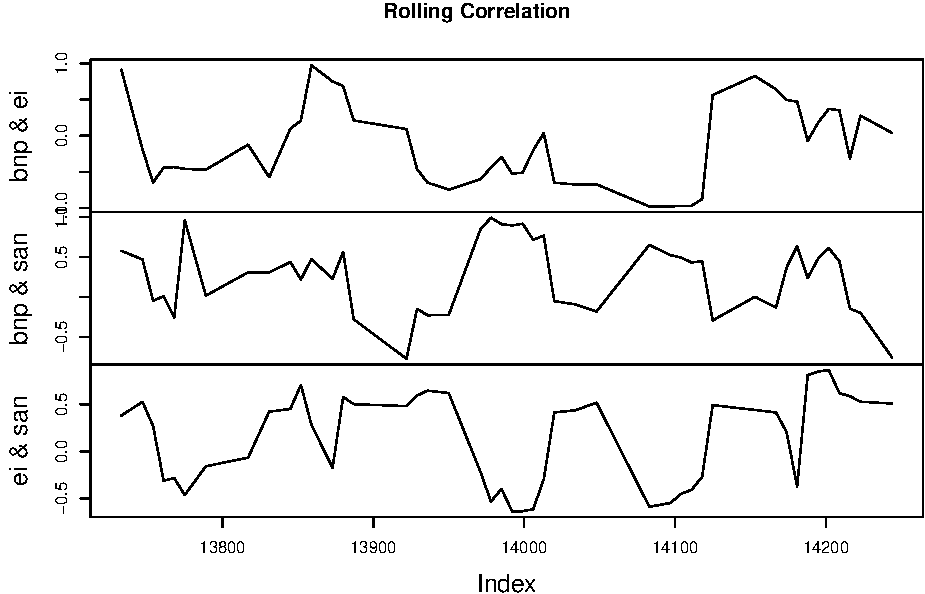
\includegraphics{TP-1_files/figure-latex/correl-roll-1.pdf}

\hypertarget{analyse-en-composantes-principales}{%
\subsection{Analyse en composantes
principales}\label{analyse-en-composantes-principales}}

\begin{itemize}
\tightlist
\item
  Effectuer une ACP de la matrice de covariance des rendements
  hebdomadaires
\end{itemize}

\begin{Shaded}
\begin{Highlighting}[]
\NormalTok{ts.hebdo }\OtherTok{\textless{}{-}}\NormalTok{ ts.all.weekly}

\NormalTok{nb.ev }\OtherTok{=} \DecValTok{6}
\NormalTok{nb.obs }\OtherTok{\textless{}{-}} \FunctionTok{nrow}\NormalTok{(ts.hebdo)}

\NormalTok{res.pca}\FloatTok{.1} \OtherTok{\textless{}{-}} \FunctionTok{prcomp}\NormalTok{(ts.hebdo, }\AttributeTok{scale=}\ConstantTok{TRUE}\NormalTok{)}

\CommentTok{\# normalized eigenvalues}
\NormalTok{norm.ev }\OtherTok{\textless{}{-}}\NormalTok{ res.pca}\FloatTok{.1}\SpecialCharTok{$}\NormalTok{sdev}\SpecialCharTok{\^{}}\DecValTok{2}
\NormalTok{norm.ev }\OtherTok{\textless{}{-}}\NormalTok{ norm.ev}\SpecialCharTok{/}\FunctionTok{sum}\NormalTok{(norm.ev)}

\NormalTok{large.ev}\FloatTok{.1} \OtherTok{\textless{}{-}}\NormalTok{ norm.ev[}\DecValTok{1}\SpecialCharTok{:}\NormalTok{nb.ev]}
\FunctionTok{names}\NormalTok{(large.ev}\FloatTok{.1}\NormalTok{) }\OtherTok{\textless{}{-}} \FunctionTok{paste}\NormalTok{(}\StringTok{"PC"}\NormalTok{, }\FunctionTok{seq\_along}\NormalTok{(large.ev}\FloatTok{.1}\NormalTok{))}


\NormalTok{plot}\FloatTok{.1} \OtherTok{\textless{}{-}} \FunctionTok{barplot}\NormalTok{(}\DecValTok{100}\SpecialCharTok{*}\NormalTok{large.ev}\FloatTok{.1}\NormalTok{, }\AttributeTok{ylim=}\FunctionTok{c}\NormalTok{(}\DecValTok{0}\NormalTok{,}\DecValTok{60}\NormalTok{), }
                  \AttributeTok{col=}\StringTok{"blue"}\NormalTok{, }\AttributeTok{ylab=}\StringTok{"Contribution (\%)"}\NormalTok{,}
                  \AttributeTok{main=}\StringTok{"Premier CP des actions du CAC40"}\NormalTok{)}
\FunctionTok{lines}\NormalTok{(plot}\FloatTok{.1}\NormalTok{, }\DecValTok{100}\SpecialCharTok{*}\FunctionTok{cumsum}\NormalTok{(large.ev}\FloatTok{.1}\NormalTok{), }\AttributeTok{type=}\StringTok{"b"}\NormalTok{, }\AttributeTok{pch=}\DecValTok{5}\NormalTok{, }\AttributeTok{col=}\StringTok{"red"}\NormalTok{, }\AttributeTok{lty=}\DecValTok{2}\NormalTok{)}
\FunctionTok{legend}\NormalTok{(}\StringTok{"right"}\NormalTok{, }\AttributeTok{legend=}\FunctionTok{c}\NormalTok{(}\StringTok{"taux de contribution"}\NormalTok{, }\StringTok{"contribution cumulée"}\NormalTok{),}
       \AttributeTok{col=}\FunctionTok{c}\NormalTok{(}\StringTok{"blue"}\NormalTok{, }\StringTok{"red"}\NormalTok{), }\AttributeTok{lty=}\DecValTok{1}\SpecialCharTok{:}\DecValTok{2}\NormalTok{, }\AttributeTok{cex=}\FloatTok{0.8}\NormalTok{) }
\end{Highlighting}
\end{Shaded}

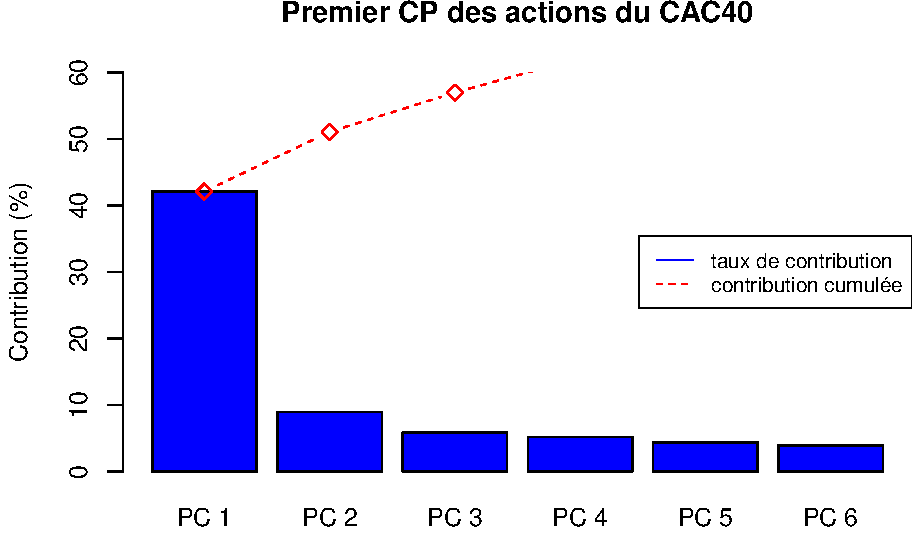
\includegraphics{TP-1_files/figure-latex/PCA-1.pdf}

\begin{itemize}
\item
  Observer les projections des variables sur les deux premiers vecteurs
  propres, et tenter de fournir une interprétation économique de ces
  facteurs.
\item
  Interprétation : D'après le graphique précédent, on remarque que 50\%
  de la contribution est expliquée par les deux premières composantes
  principales. Ce qui veux dire que 50\% du risque de l'indice du CAC40
  (40\% au risque pour la première et environ 10\% du risque pour la
  seconde) est expliquée par les deux premiers axes . Ce qui nous ammène
  à dire que la diversification dans l'indice CAC40 n'est pas à priori
  la meilleure solution . Donc l'investissement sur un nombre plus
  faible d'actif de l'indice ne nous exclut pas à l'exposition du risque
  puisque nous avons 50\% de risque dans l'indice.
\item
  Projection sur la première composante principale
\end{itemize}

\begin{Shaded}
\begin{Highlighting}[]
\NormalTok{v }\OtherTok{\textless{}{-}}\NormalTok{ res.pca}\FloatTok{.1}\SpecialCharTok{$}\NormalTok{rotation[,}\DecValTok{1}\NormalTok{]}
\NormalTok{knitr}\SpecialCharTok{::}\FunctionTok{kable}\NormalTok{(v[}\FunctionTok{order}\NormalTok{(}\FunctionTok{abs}\NormalTok{(v), }\AttributeTok{decreasing=}\NormalTok{T)][}\DecValTok{1}\SpecialCharTok{:}\DecValTok{10}\NormalTok{], }\AttributeTok{format=}\StringTok{"latex"}\NormalTok{, }\AttributeTok{booktabs=}\NormalTok{T, }
    \AttributeTok{caption=}\StringTok{"Projection des rendements sur la 1ème CP"}\NormalTok{, }\AttributeTok{col.names=}\StringTok{"Corrélation"}\NormalTok{) }
\end{Highlighting}
\end{Shaded}

\begin{table}

\caption{\label{tab:unnamed-chunk-1}Projection des rendements sur la 1ème CP}
\centering
\begin{tabular}[t]{lr}
\toprule
  & Corrélation\\
\midrule
sgo.pa & -0.2170328\\
ker.pa & -0.2105551\\
cs.pa & -0.2063743\\
gle.pa & -0.2039229\\
ri.pa & -0.1951147\\
\addlinespace
mc.pa & -0.1934976\\
ac.pa & -0.1902769\\
dg.pa & -0.1874261\\
ml.pa & -0.1852249\\
edf.pa & -0.1826654\\
\bottomrule
\end{tabular}
\end{table}

On peut interpréter le premier axe factoriel comme un facteur de
rendement lié aux domaines de la banque, le luxe,matériaux de
construction, distribution de vin.

\end{document}
